\documentclass[margin=2pt]{standalone}

\usepackage{amsmath,amsfonts}
\usepackage{booktabs}
\usepackage{multirow}
\usepackage{colortbl}
\usepackage{natbib}
\usepackage[dvipsnames]{xcolor}
\usepackage{tikz}
\usepackage{newtxmath}
\usepackage{newtxtext,newtxmath}

\usetikzlibrary{positioning}
\usetikzlibrary{arrows}
\usetikzlibrary{calc,fit}
\usetikzlibrary{shapes.geometric}
\usetikzlibrary{shapes.misc}
\usetikzlibrary{decorations.pathmorphing}
\usetikzlibrary{decorations.pathreplacing}



\begin{document}
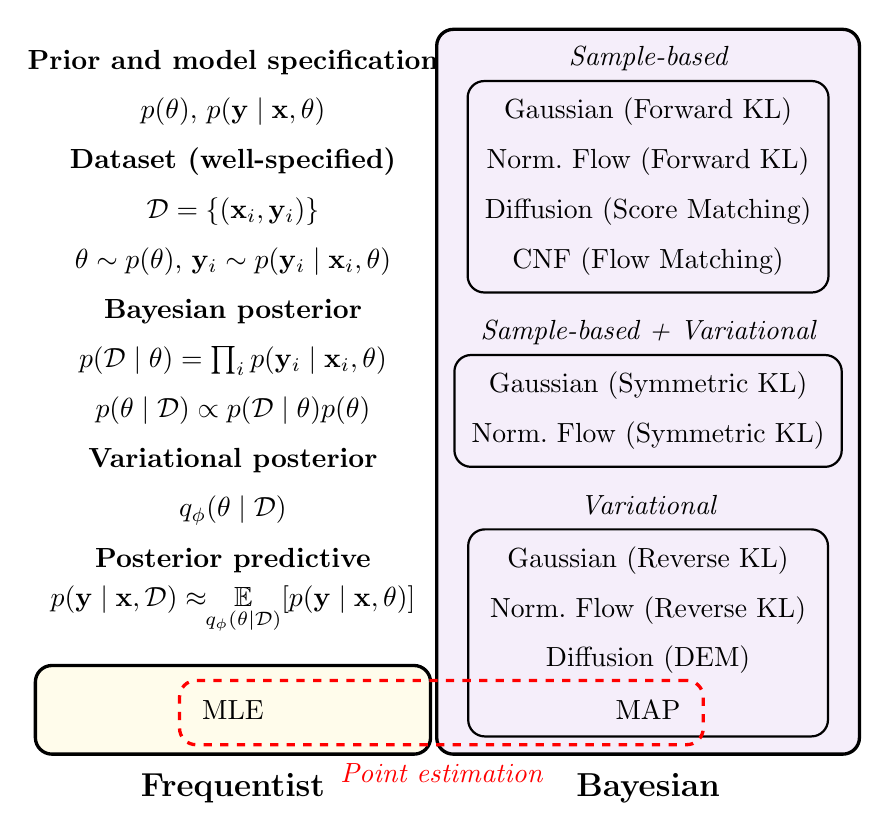
\begin{tikzpicture}[
    every node/.style={inner sep=0pt},
    algo/.style={},
    group/.style={draw, rounded corners=6pt, thick, inner sep=6pt, minimum width=130pt},
    crossgroup/.style={draw, rounded corners=6pt,inner sep=8pt, very thick, dashed},
    biggroup/.style={draw, rounded corners=6pt, very thick, inner sep=6pt, minimum width=140pt},
    y=18pt, 
    x=150pt]

\definecolor{bayescolor}{HTML}{9b59d0}
\definecolor{freqcolor}{HTML}{ffe433}

\pgfdeclarelayer{background}
\pgfsetlayers{background,main}

\node[algo] (algo_gaussian_forward) at (0,0) {Gaussian (Forward KL)};
\node[algo] (algo_nf_forward) at (0,-1) {Norm.\ Flow (Forward KL)};
\node[algo] (algo_dsm) at (0,-2) {Diffusion (Score Matching)};
\node[algo] (algo_fm) at (0,-3) {CNF (Flow Matching)};
\node[group, fit=(algo_gaussian_forward) (algo_nf_forward) (algo_dsm) (algo_fm)] (group_sample) {};

\node[algo] (algo_gaussian_sym) at (0,-5.5) {Gaussian (Symmetric KL)};
\node[algo] (algo_nf_sym) at (0,-6.5) {Norm.\ Flow (Symmetric KL)};
\node[group, fit=(algo_gaussian_sym) (algo_nf_sym)] (group_sym) {};

\node[algo] (algo_gaussian_reverse) at (0,-9) {Gaussian (Reverse KL)};
\node[algo] (algo_nf_reverse) at (0,-10) {Norm.\ Flow (Reverse KL)};
\node[algo] (algo_dem) at (0,-11) {Diffusion (DEM)};
\node[algo] (algo_map) at (0,-12) {MAP};
\node[group, fit=(algo_gaussian_reverse) (algo_nf_reverse) (algo_dem) (algo_map)] (group_variational) {};

\node[algo] (algo_mle) at (-1,-12) {MLE};

\node[above=3pt of group_sample] (group_sample_title) {\it Sample-based};
\node[above=3pt of group_sym] {\it Sample-based + Variational};
\node[above=3pt of group_variational] {\it Variational\vphantom{p}};

\node[group, fit=(algo_mle), draw=none] (group_frequentist) {};

\begin{pgfonlayer}{background}
    \node[biggroup, fill=freqcolor!10, fit=(group_frequentist)] (biggroup_frequentist) {};
    \node[biggroup, fill=bayescolor!10, fit=(group_sample_title) (group_sym) (group_variational)] (biggroup_bayesian) {};
\end{pgfonlayer}

\node[below=6pt of biggroup_frequentist] {\bf\large Frequentist};
\node[below=6pt of biggroup_bayesian] {\bf\large Bayesian};

\node[crossgroup, fit=(algo_map) (algo_mle),yshift=-1pt,draw=red] (group_point) {};
\node[below=6pt of group_point] {\it\color{red} Point estimation};



\node[algo] (prior) at (-1,-0) {$p(\theta)$, $p(\mathbf{y}\mid\mathbf{x},\theta)$};
\node[algo] at (-1,1) {\bf Prior and model specification};

\node[algo] (dataset) at (-1,-2) {$\mathcal{D}=\left\{(\mathbf{x}_i,\mathbf{y}_i)\right\}$};
\node[algo] (dataset_iid) at (-1,-3) {$\theta\sim p(\theta)$, $\mathbf{y}_i\sim p(\mathbf{y}_i\mid \mathbf{x}_i,\theta)$};
\node[algo] at (-1,-1) {\bf Dataset (well-specified)};

\node[algo] (likelihood) at (-1,-5) {$p(\mathcal{D}\mid\theta)=\prod_i p(\mathbf{y}_i\mid\mathbf{x}_i,\theta)$};
\node[algo] (posterior) at (-1,-6) {$p(\theta\mid\mathcal{D})\propto p(\mathcal{D}\mid\theta)p(\theta)$};
\node[algo] at (-1,-4) {\bf Bayesian posterior};

\node[algo] (varposterior) at (-1,-8) {$q_\phi(\theta\mid\mathcal{D})$};
\node[algo] at (-1,-7) {\bf Variational posterior};

\node[algo] (postpred) at (-1,-10) {$p(\mathbf{y}\mid\mathbf{x},\mathcal{D})\approx\!\!\operatorname*{\mathbb{E}}\limits_{q_\phi(\theta\mid\mathcal{D})}[p(\mathbf{y}\mid\mathbf{x},\theta)]$};
\node[algo] at (-1,-9) {\bf Posterior predictive};

\end{tikzpicture}
\end{document}